\begin{frame}
	\frametitle{Linear regression models}
	
	\begin{itemize}
		 \item Single level regression model; ordinary least squares (OLS)
		 \item Linear change in the data given a predictor variable 
		 \item Predictor can be continuous (e.g. frequency: 0 -- 100) or discrete (e.g. frequency: high vs.~low)
		 \item Allows multiple predictors 
	\end{itemize}

\end{frame}	


\begin{frame}
	\frametitle{Linear regression models}
	
	\begin{equation}
		y_i = \alpha + \beta \times x_{i} + \epsilon_i
%		y = \alpha + \beta \times x + \epsilon
	\end{equation}

\begin{minipage}{.4\textwidth}
	\begin{itemize}
		\item $y$: data
		\item $\alpha$: intercept
		\item $\beta$: slope (gradient)
		\end{itemize}
\end{minipage}
\hfill
\begin{minipage}{.5\textwidth}
	\begin{itemize}
		\item $x$: predictor
		\item $\epsilon$: residual error (i.e. noise)
	\end{itemize}
\end{minipage}
	\begin{equation}
		\epsilon_i \sim N(0,\sigma^2)
%		\epsilon \sim N(0,\sigma^2)
	\end{equation}
	
	\begin{itemize}
		\item $R$ function $lm()$ (part of the base $R$ package)
		\item Syntax: $lm($ \texttt{outcome variable} $\sim$ \texttt{predictor} $,$ \texttt{data frame} )
		\item Your turn: see $R$ script $exercise\_lm.R$
	\end{itemize}
	
\end{frame}


\begin{frame}[fragile]
	\frametitle{Linear regression models}
	
	\begin{minipage}{.55\textwidth}
	\begin{figure}		
		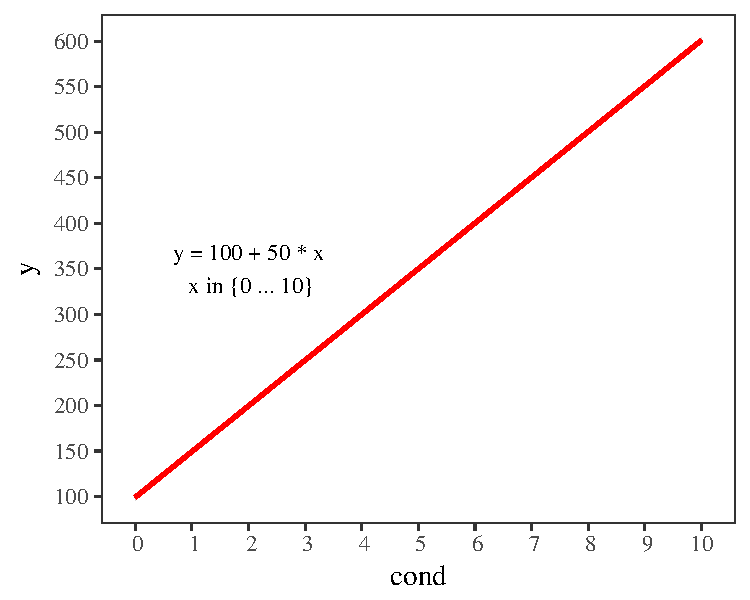
\includegraphics[scale= .5]{gfx/lm.pdf}
		\caption{Predictor $x$ is continuous}
	\end{figure}
	\end{minipage}
\hfill
	\begin{minipage}{.35\textwidth}
		\begin{verbatim}
			> head(data)
			  cond        y
			     9 465.8291
			     0 108.5086
			     9 569.3380
			     7 431.7700
			     7 449.9238
			     3 233.3673
		\end{verbatim}
	\end{minipage}
		
\end{frame}




\begin{frame}[fragile]
	\frametitle{Linear regression models}

	\begin{minipage}{.55\textwidth}	
	\begin{figure}		
		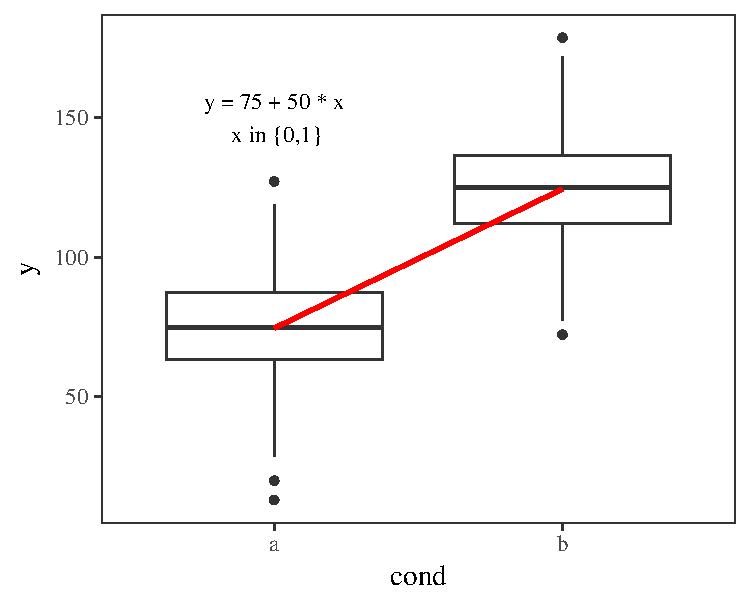
\includegraphics[scale= .5]{gfx/lmdiscrete.pdf}
		\caption{Predictor $x$ is discrete}
	\end{figure}
	\end{minipage}
	\hfill
	\begin{minipage}{.35\textwidth}
		\begin{verbatim}

				> head(data)
				  cond         y
				     b 105.10129
				     a  82.73471
				     b 104.00330
				     b  97.21434
				     b 101.53576
				     a  68.83296
		
			\end{verbatim}
		\end{minipage}

%	\begin{itemize}
%		\item Aside: Data points outside the 25th and 75th percentiles are often considered outliers. However, the present data are simulated and come from a \textit{know} population that is normal distribution.		
%	\end{itemize}
	
\end{frame}


\begin{frame}[fragile]
	\frametitle{Linear regression models}
	See script $LM\_model\_discrete.R$
	\begin{verbatim}
	
> data %>% 
+   group_by(cond) %>%
+   summarise (mean = mean(y),
+              sd = sd(y))
# A tibble: 2 x 3
    cond      mean       sd
  <fctr>     <dbl>    <dbl>
1      a  74.49868 18.09908
2      b 124.44140 17.30632
	
	\end{verbatim}
	Population means are 75 for $cond$ $a$ and 125 for $cond$ $b$.
	
\end{frame}

\begin{frame}[fragile]
	\frametitle{Linear regression models}
	
	\begin{verbatim}
	> m <- lm(y ~ cond, data)
	> summary(m)$coef
	\end{verbatim}
	
	\begin{table}[!htbp] \centering 
		\begin{tabular}{@{\extracolsep{5pt}} ccccc} 
			\\[-1.8ex]\hline 
			& Estimate & Std. Error & t value & Pr(\textgreater \textbar t\textbar ) \\ 
			\hline \\[-1.8ex] 
			(Intercept) & $74.499$ & $0.804$ & $92.626$ & $< 0.001$ \\ 
			condb & $49.943$ & $1.120$ & $44.605$ & $< 0.001$ \\ 
			\hline \\[-1.8ex] 
		\end{tabular} 
	\end{table} 
	
	\begin{itemize}
		\item (Intercept): y-value for $cond$ = 0; here condition $a$
		\item \texttt{condb}: change from condition $a$ (i.e. intercept) to  $b$
		\item condition $b$ + intercept is $t$ $\times$ $Std.~Error$ away from intercept 
		\item Is that what we want?
	\end{itemize}
	
\end{frame}

\begin{frame}[fragile]
	\frametitle{Linear regression models}

		\begin{itemize}
			\item Treatment contrast (default): change from intercept
		\end{itemize}	

			\begin{verbatim}			
			> contrasts(data$cond)
  b
			a 0
			b 1
			\end{verbatim}

		\begin{itemize}
			\item Sum contrast (effect magnitude): difference between $a$ and $b$
		\end{itemize}	
		
		\begin{verbatim}			
			> contrasts(data$cond) <- c(-.5, .5)
			> colnames(contrasts(data$cond)) <- c("b-a")
			> contrasts(data$cond)
			   b-a
			a -0.5
			b  0.5
		
		\end{verbatim}
			
		
	
\end{frame}


\begin{frame}[fragile]
	\frametitle{Linear regression models}


	\begin{table}[!htbp] \centering
			\caption{Treatment contrast} 
			\label{}  
		\begin{tabular}{@{\extracolsep{5pt}} ccccc} 
			\\[-1.8ex]\hline 
			& Estimate & Std. Error & t value & Pr(\textgreater \textbar t\textbar ) \\ 
			\hline \\[-1.8ex] 
			(Intercept) & $74.499$ & $0.804$ & $92.626$ & $< 0.001$ \\ 
			condb & $49.943$ & $1.120$ & $44.605$ & $< 0.001$ \\ 
			\hline \\[-1.8ex] 
		\end{tabular} 
	\end{table} 

\begin{table}[!htbp] \centering 
	\caption{Sum contrast} 
	\label{} 
	\begin{tabular}{@{\extracolsep{5pt}} ccccc} 
		\\[-1.8ex]\hline 
		& Estimate & Std. Error & t value & Pr(\textgreater \textbar t\textbar ) \\ 
		\hline \\[-1.8ex] 
		(Intercept) & $99.470$ & $0.560$ & $177.678$ & $< 0.001$ \\ 
		condb-a & $49.943$ & $1.120$ & $44.605$ & $< 0.001$ \\ 
		\hline \\[-1.8ex] 
	\end{tabular} 
\end{table} 

\end{frame}

\begin{frame}[fragile]
	\frametitle{Linear regression models}
	\begin{itemize}
		\item Estimation of effect magnitude
		\item Linear function can account for and predict unobserved data 
		\item Can account for additional sources of variance and potentially confounding variable by adding those to the model (co-variates)
		\item However, data are more complex than that:
		\item[] E.g. multiple observation per participant/item
		\item Solution: Linear mixed effects models 
	\end{itemize}

\end{frame}

